\chapter{Zusammenarbeit und soziale Funktion}
\label{ch:zusammenarbeit}

\section{Freunde}% Screenshot von beiden Seiten (Menü und nutzerseite)
\label{sec:freunde}
PUMA bietet die Möglichkeit, andere Nutzer als Freunde zu kennzeichnen. Freundschaften\index{Freunde} ermöglichen das Teilen von Publikationen und Lesezeichen. Dazu in der Sichtbarkeitseinstellung eines Eintrags \enquote{andere} und dann \enquote{friends} auswählen, dann können \enquote{Freunde} diesen Eintrag sehen. Einen Überblick über Einträge, die für \enquote{Freunde} sichtbar sind, erhält man über den Menüeintrag \enquote{meinPUMA} (\autoref{subsec:meinPuma}) unter \enquote{Einträge von Freunden} bzw. \enquote{Einträge für Freunde}.\newline

\subsection{Freund hinzufügen}
\label{subsec:freundHinzu}

Um Freunde hinzuzufügen, entweder auf den Benutzernamen unter einem Eintrag klicken, im Suchfeld auf Benutzer einschränken oder in der allgemeinen Suche user:Benutzername eingeben (\autoref{sec:suche}).Die Seite des Nutzers wird angezeigt, auf der alle öffentlichen Einträge zu sehen sind. In der rechten Menüleiste wird der Name eingeblendet, darunter besteht die Möglichkeit diesen Nutzer als Freund hinzuzufügen.
    
		
		%\begin{figure}[h!]
 %\centering
 %\fbox{\includegraphics[width=5cm]{Bilder/Kapitel8/Benutzername_in_Eintrag}}
 %\caption{Benutzername anklicken}
 %\label{fig:benutzerAnklicken}
%\end{figure}

		\begin{figure}[h!]
 \centering
 \fbox{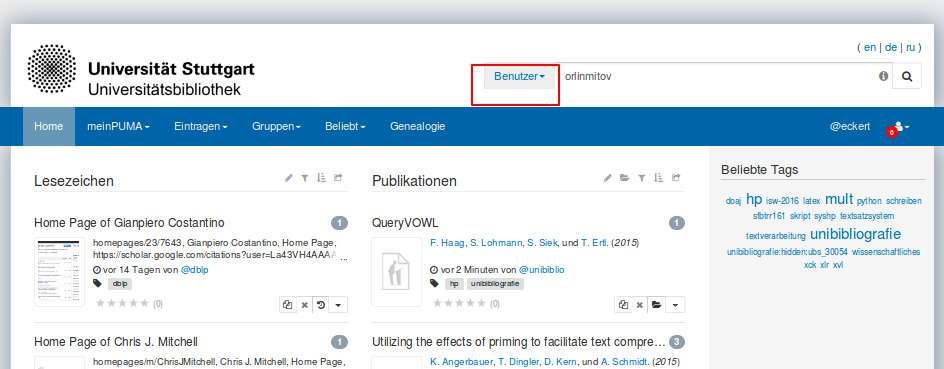
\includegraphics[width=11cm]{Bilder/Kapitel8/Benutzer_suchen}}
 \caption{Benutzer suchen}
 \label{fig:benutzerSuchen}
\end{figure}

\begin{figure}[h!]
 \centering
 \fbox{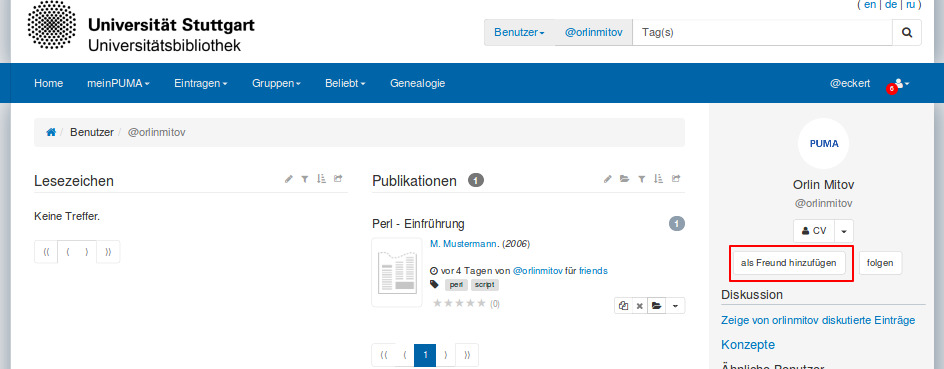
\includegraphics[width=11cm]{Bilder/Kapitel8/Nutzerseite}}
 \caption{Die Nutzerseite}
 \label{fig:nutzerseite}
\end{figure}

\subsection{Freundesübersicht}
\label{subsec:freundesuebersicht}
Die Freundesübersicht bietet einen Überblick über Freunde in PUMA. Diese Übersicht ist im Dropdown-Menü des Personensymbols. Unter dem Reiter \enquote{Freunde} erhält man einen Überblick über Freunde und kann sehen, welche Nutzer einen als Freund angegeben hat. Am Ende der Seite sind alle Publikationen aufgelistet, die mit Freunden geteilt wurden oder Freunde geteilt haben.\newline

\begin{figure}[h!]
 \centering
 \fbox{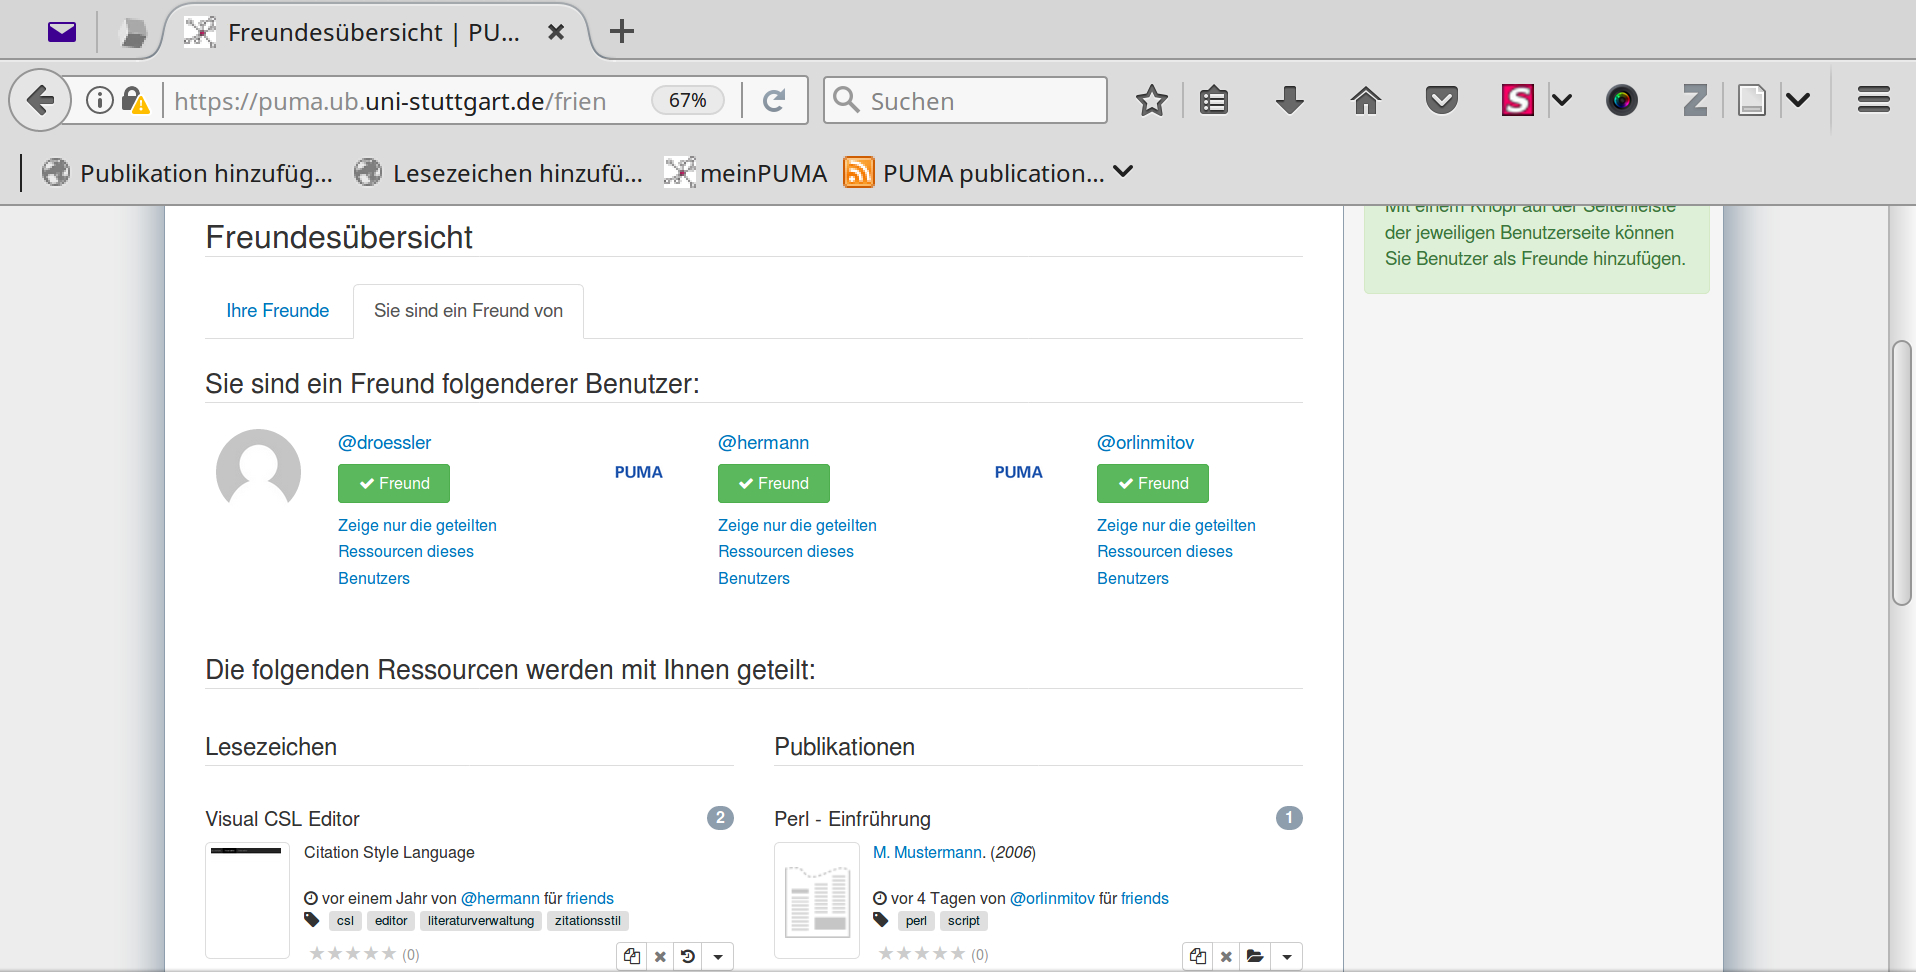
\includegraphics[width=11cm]{Bilder/Kapitel8/Freundesuebersicht}}
 \caption{Freundesübersicht}
 \label{fig:freundesuebersicht}
\end{figure}

Es besteht jederzeit die Möglichkeit, Freunde wieder zu entfernen. Hierfür mit der Maus auf den jeweiligen grünen Kasten \enquote{Freund} des Freundes, der entfernt werden soll, klicken.

\section{Gruppen}
\label{sec:gruppen}
Gruppen\index{Gruppen} ermöglichen eine gemeinsame Literatursammlung und erleichtern so die Umsetzung von gemeinsamen Projekten. Gleichzeitig können innerhalb einer Gruppe Volltext getauscht werden.

\subsection{Gruppen \index{Gruppen!beitreten}suchen und beitreten}
\label{subsec:gruppenSuchenBeitreten}

\begin{figure}[h!]
 \centering
 \fbox{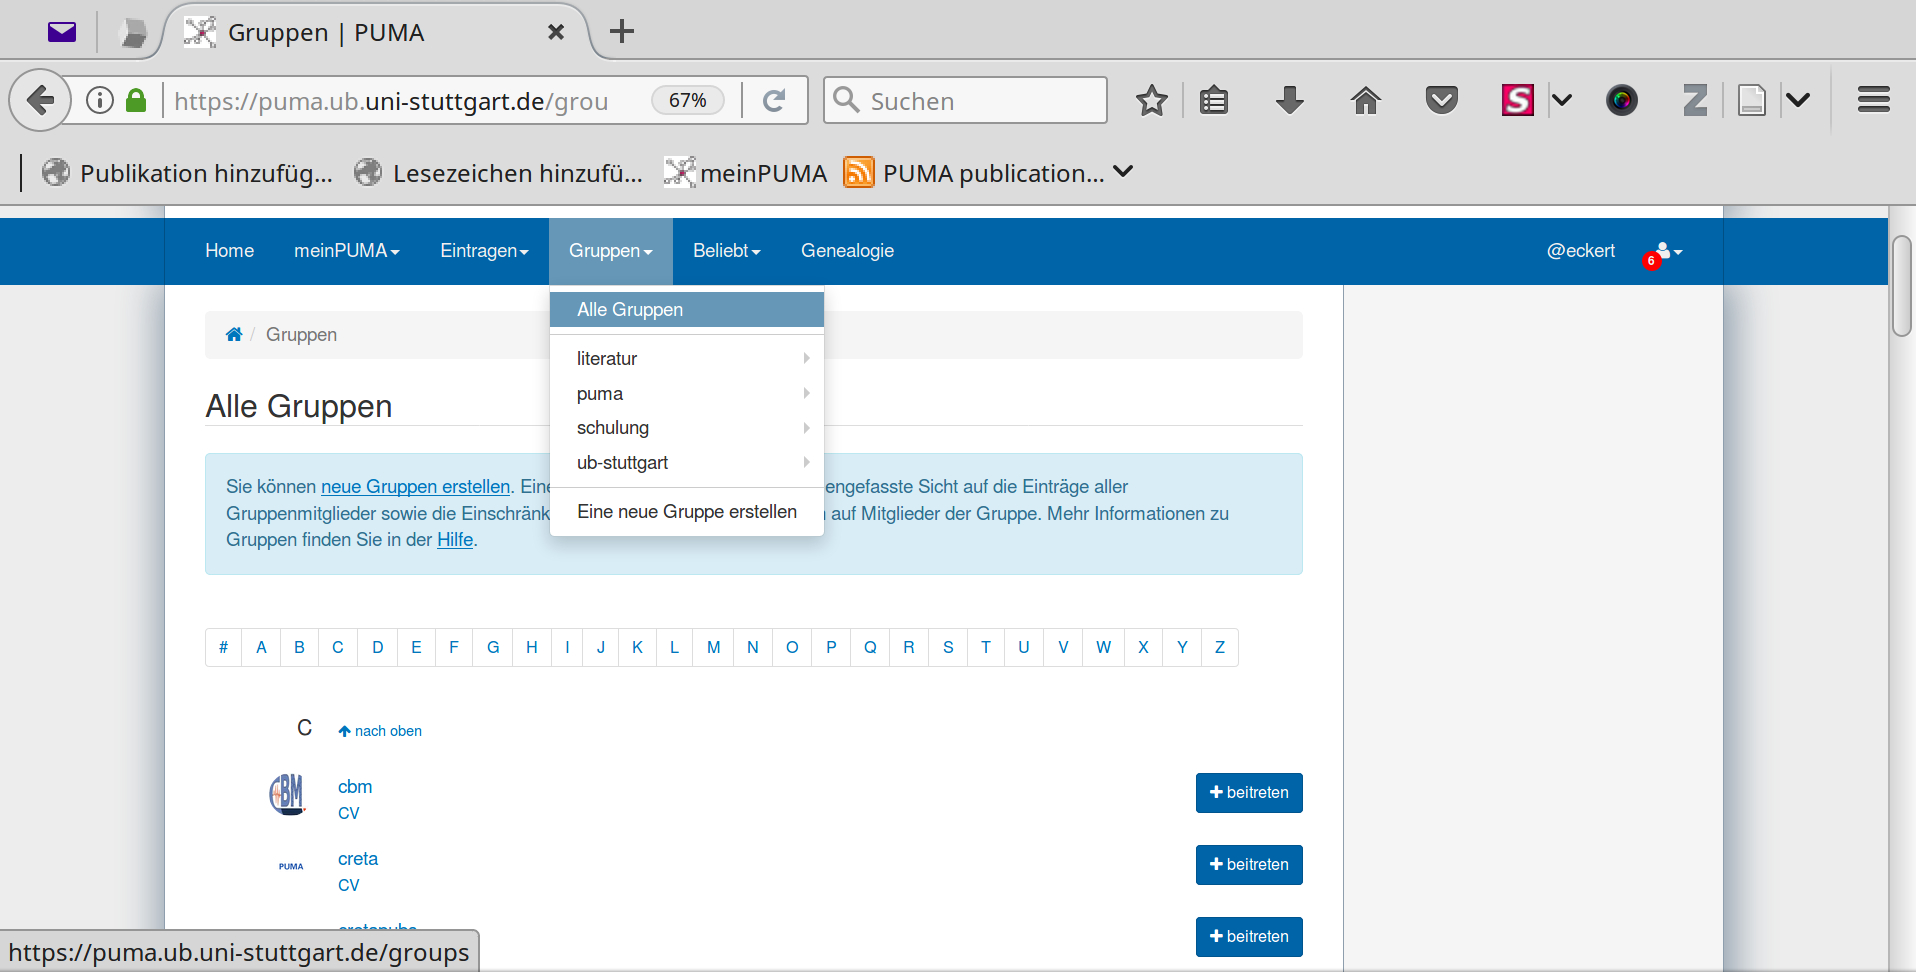
\includegraphics[width=11cm]{Bilder/Kapitel8/Gruppen-Uebersichtsseite}}
 \caption{Allgemeine Liste}
 \label{fig:allgemeineListe}
\end{figure}

Unter dem Hauptmenü \enquote{Gruppen} im Dropdown-Menü auf \enquote{Alle Gruppen} gehen. Es öffnet sich eine Übersicht über alle Gruppen bei PUMA in alphabetischer Reihenfolge. Rechts neben dem jeweiligen Gruppennamen befindet sich ein Button, um der Gruppe beizutreten. Wenn es eine offene Gruppe ist, kann man der gewünschten Gruppe beitreten. In das Feld \enquote{Begründung} kann eingegeben werden, warum man der Gruppe beitreten möchte. Um zu verhindern, dass Programme automatisiert Gruppen beitreten, wird ein Captcha-Abfrage duchgeführt. Nach Abschluss durch \enquote{Anfrage absenden} werden die Gruppen-Administrator über das Beitretungsgesuch per E-Mail benachrichtigt.
	
\begin{figure}[h!]
 \centering
 \fbox{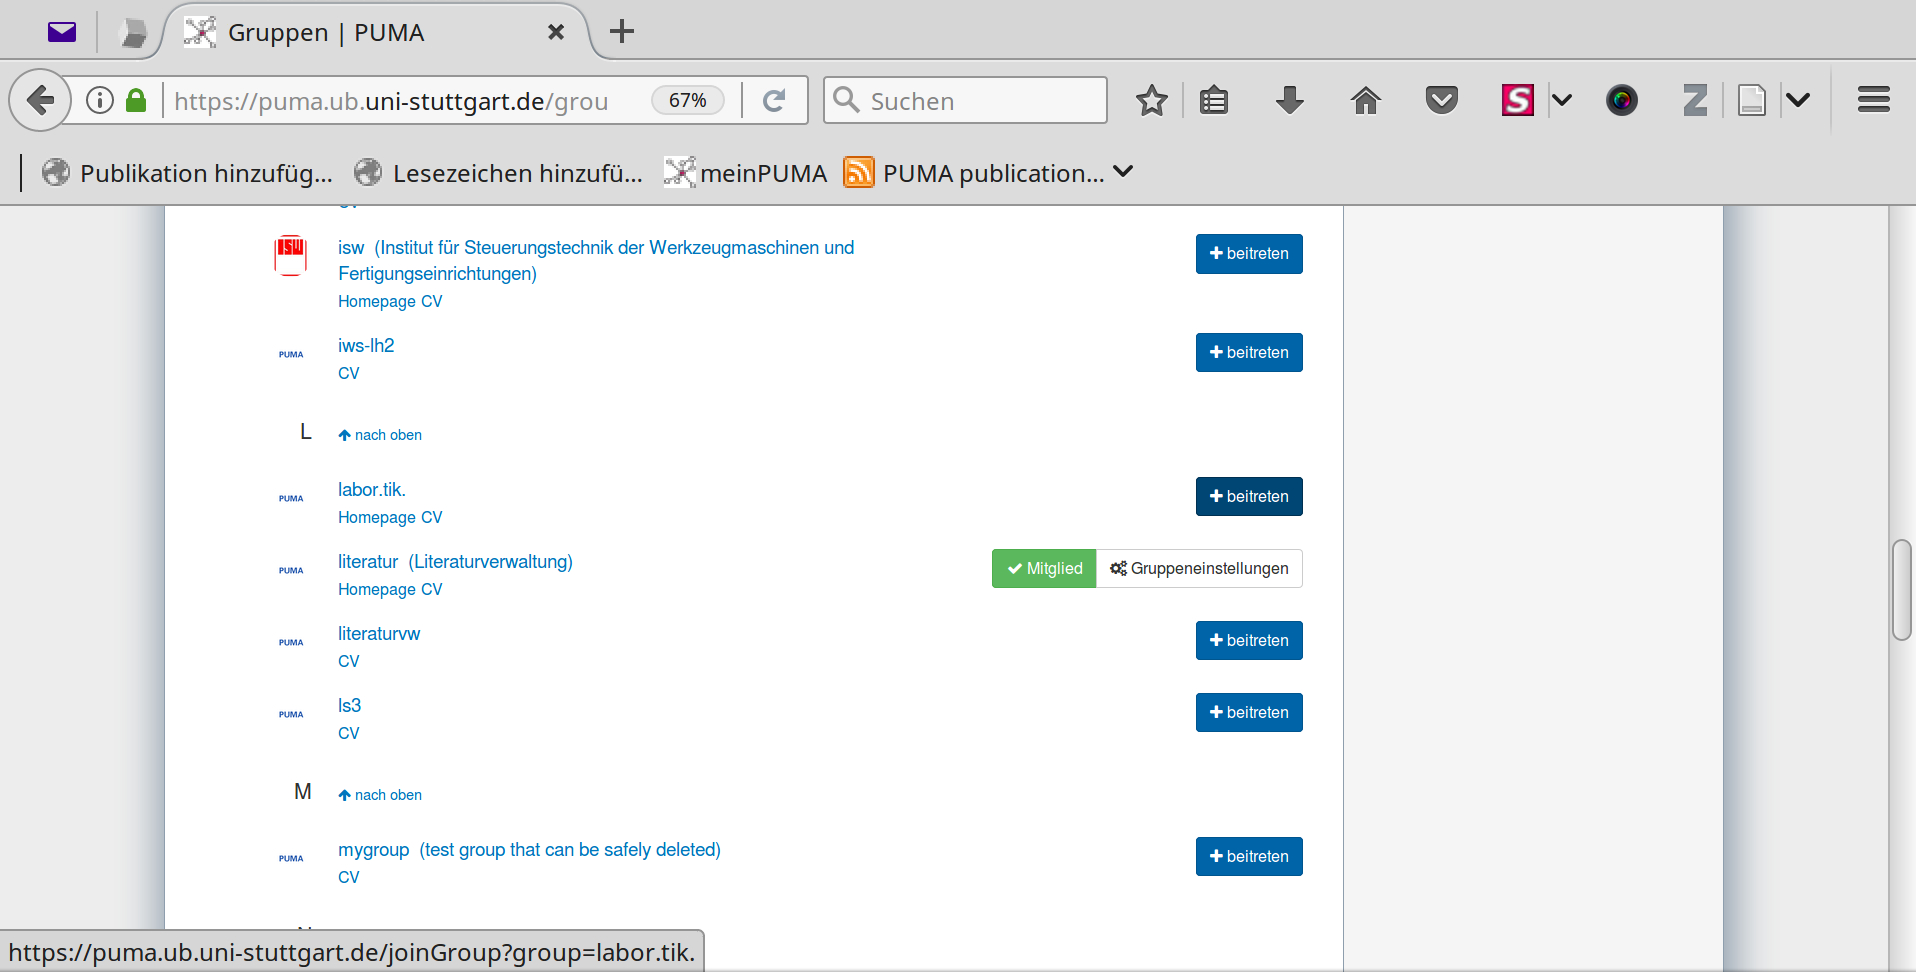
\includegraphics[width=11cm]{Bilder/Kapitel8/Beitreten_einer_Gruppe}}
 \caption{Beitreten einer Gruppe}
 \label{fig:gruppeBeitreten}
\end{figure}

Ein Gruppenadministrator kann nun den Nutzer aufnehmen, seine Rolle festlegen oder dessen Beitrittsanfrage ablehnen.
\subsection{Gruppen erstellen\index{Gruppen!erstellen}}
\label{subsec:gruppenErstellen}

Im Hauptmenü auf \enquote{Gruppen} im Dropdown-Menü unter \enquote{Eine neue Gruppe erstellen} den Gruppennamen und optional eine Beschreibung der Gruppe eingeben.


\begin{figure}[h!]
 \centering
 \fbox{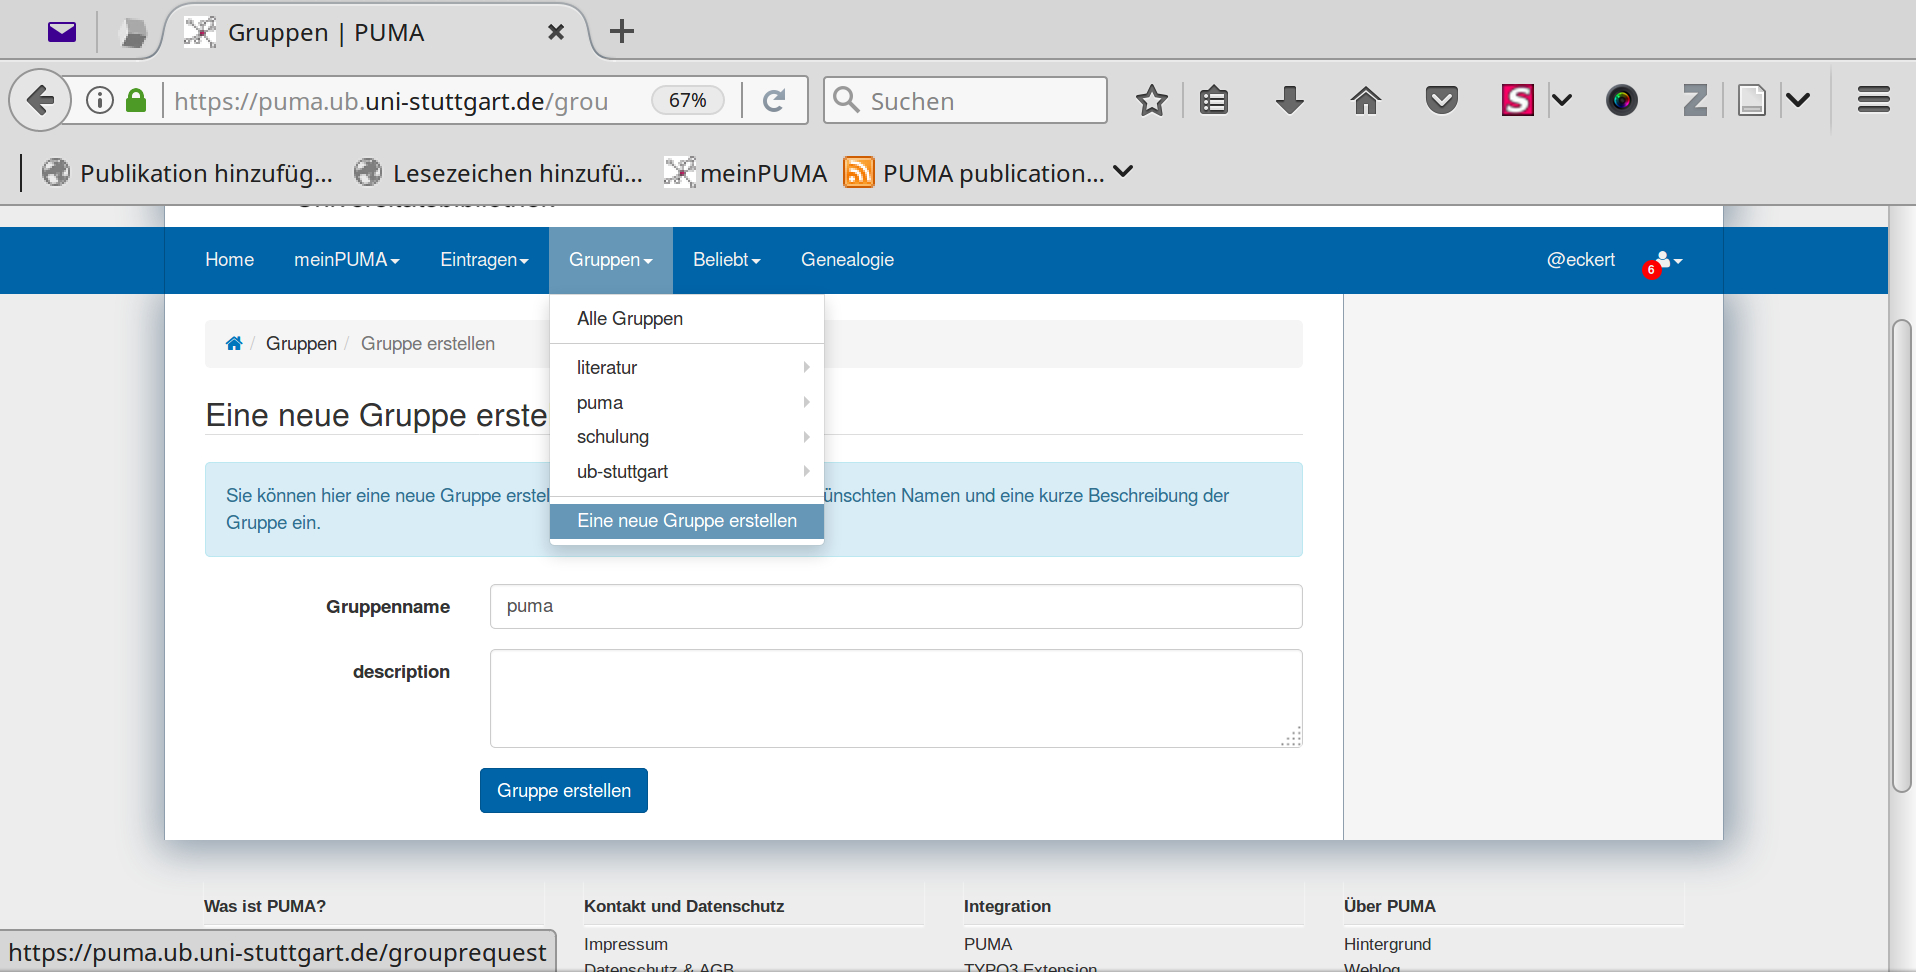
\includegraphics[width=11cm]{Bilder/Kapitel8/Neue_Gruppe_erstellen}}
 \caption{Erstellung einer neuen Gruppe}
 \label{fig:erstellungNeueGruppe}
\end{figure}

Die neu angelegte Gruppe kann nun beim Eintragen einer neuen Publikation oder eines neuen Lesezeichens ausgewählt werden, indem bei der Sichtbarkeit\index{Sichtbarkeit} unter dem Punkt \textit{andere} diese ausgewählt wird.
\subsection{Die Gruppenseite}
\label{subsec:gruppenseite}
Die Gruppenseite \index{Gruppen} gibt einen Überblick über alle Lesezeichen und Publikationen der Mitglieder, die in der Gruppe angemeldet sind. Im Dropdown-Menü \enquote{Gruppen} werden alle Gruppen gelistet, bei denen man Mitlied ist. Einen Überblick über alle in PUMA angelegten Gruppen erhält man unter \enquote{alle Gruppen}, auch diese können ausgewählt werden.%Screenshot
\newline\newline
Funktionen auf der Gruppenseite:
\begin{figure}[h!]
 \centering
 \fbox{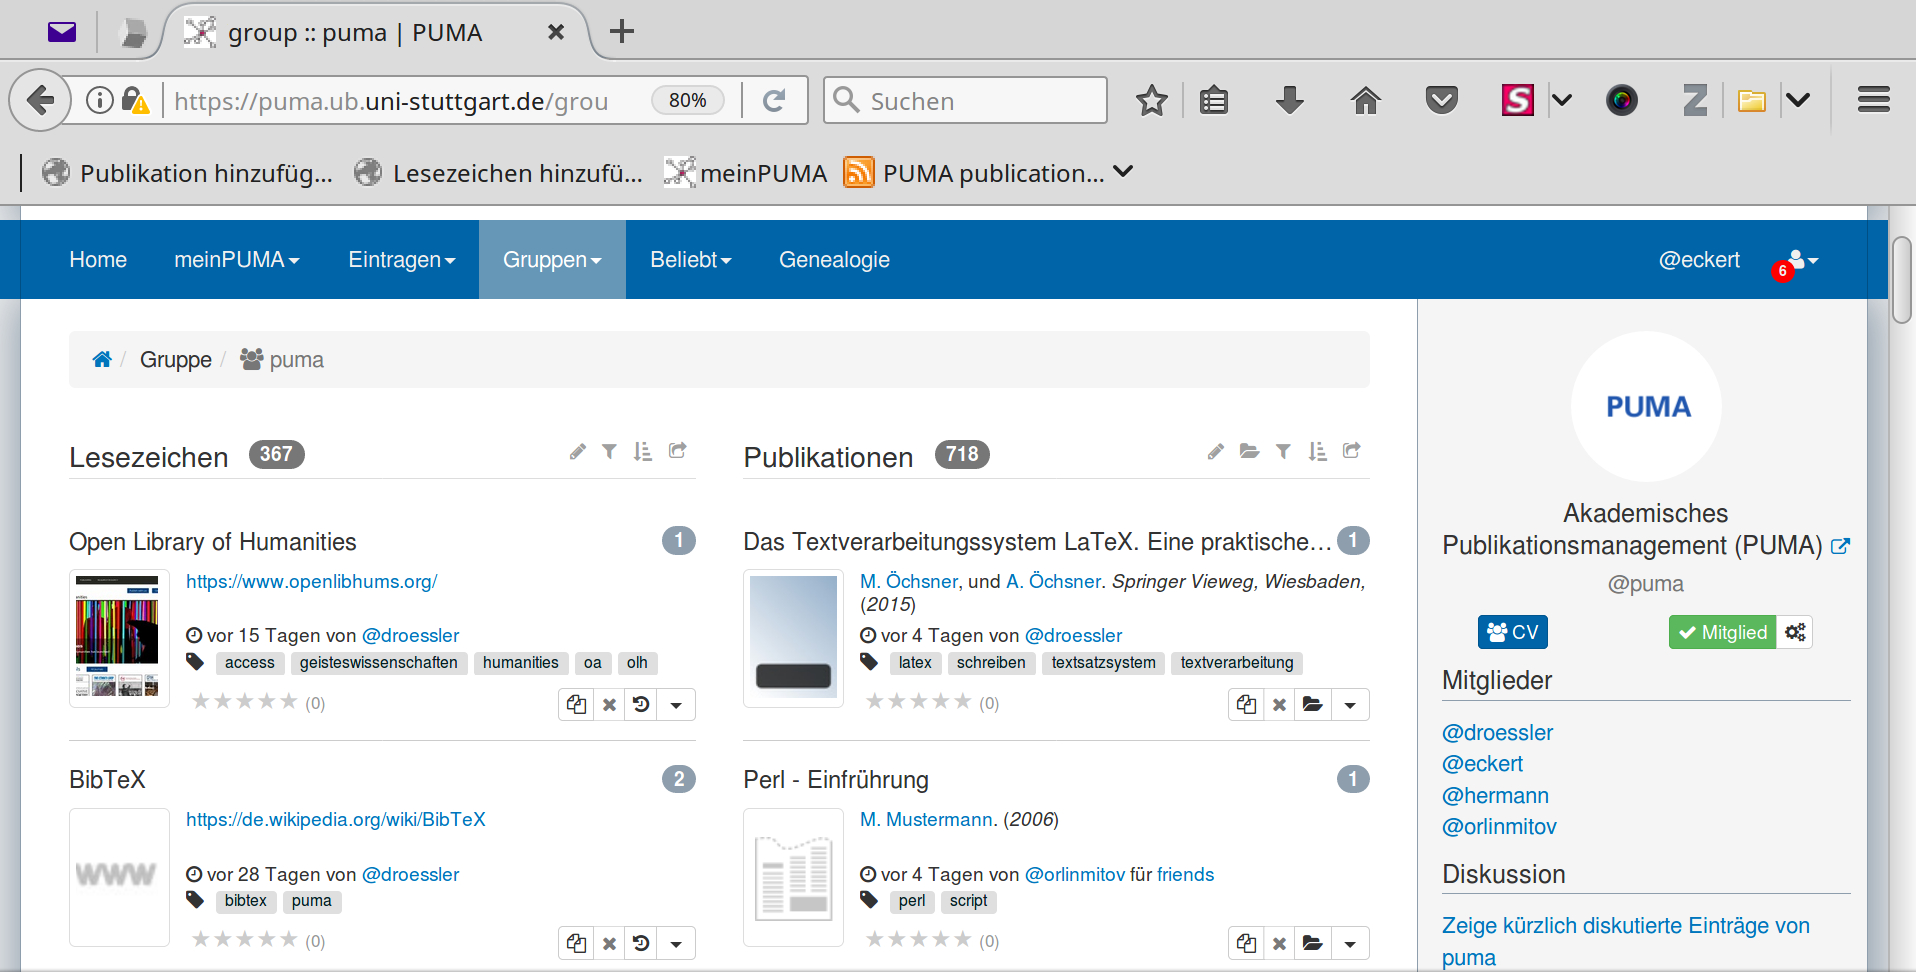
\includegraphics[width=11cm]{Bilder/Kapitel8/Gruppenseite}}
 \caption{Die Gruppenseite}
 \label{fig:gruppenseite}
\end{figure}
\begin{description}
\item [CV/Lebenslauf der Gruppe] \hfill \\
Über den CV-Button auf der rechten Seite wird eine Seite aufgerufen, auf der die Gruppe näher beschrieben wird. Es können drei verschiedene Layouttypen vom Gruppenadmin ausgewählt werden. In der Standardeinstellung werden alle Publikationen und Lesezeichen, die von einem Gruppenmitglied mit myown getaggt wurden gelistet. \todo[inline]{näher beschreiben bzw. verweisen}
\item [Mitglieder-Liste] \hfill \\
Unterhalb des Gruppenbildes befindet sich die Liste aller Mitglieder. 
\item [Diskussionen] Um sich einen Überblick über die diskutierten Einträge zu verschaffen, klicken Sie unter dem Abschnitt Diskussion auf der rechten Seite auf \enquote{Zeige kürzlich diskutierte Einträge von PUMA}. 
\end{description}
 \todo[inline]{es fehlt wie das Bild eingegeben werden kann, Verweise auf Homepage}
\subsection{Rollen in einer Gruppe}
\label{subsec:RollenInGruppe}
In PUMA werden drei Rollen unterschieden:
\begin{description}
    \item [Administrator\index{Administrator}:] kann Einstellungen der Gruppenseite und das Layout des Gruppenlebenslaufes editieren. Einträge, die mit dem Systemtag \ref{} \textit{for:gruppenname} \ref{subsec:gruppenfunktion} an die Gruppe gesendet werden, können nur von Gruppenadministratoren bearbeitet werden. Mit der Administratorrolle können neue Mitglieder eingeladen und vorhandene ausgeladen sowie die Rollen der anderen Mitglieder verändert (z.B. weiteren Administrator ernennen) werden.
    \item [Moderator\index{Moderator}:] hat Zugriff auf die Mitgliederliste und kann andere Nutzer in die Gruppe einladen und die eigene Rolle auf \textit{Nutzer} herabsetzen.
    \item [Nutzer\index{Nutzer}:] ist ein Mitglied der Gruppe und hat keine Befugnisse, in der Gruppe Änderungen oder neue Einstellungen vorzunehmen.
\end{description}

\subsection{Einträge für eine Gruppe}
\label{subsec:gruppenfunktion}
Sobald ein Nutzer Mitglied einer Gruppe ist, werden seine öffentlichen Einträge automatisch in der Sammlung der Gruppe angezeigt. Die anderen Mitglieder können diese Publikation aber erst bearbeiten wenn sie die Publikation in die eigene Sammlung übertragen. Eine weitere Möglichkeit, eine Publikation in die Gruppensammlung zu übertragen, bietet das Gruppenoptionsfeld. Damit kann beim Eintragen der Publikation eine Gruppe ausgewählt werden, für die die Publikation interessant ist. Auch diese Einträge können erst dann von den Mitgliedern bearbeitet werden, wenn sie in die eigene Sammlung aufgenommen werden.
\todo[inline]{Wird der Unterschied zwischen sichtbar und interessant irgendwo beschrieben?}
Um gemeinsame Einträge erstellen zu können, besteht die Möglichkeit, beim Eintragen der Publikation den Systemtag \textit{for:gruppenname} einzugeben. Der Eintrag erscheint wie alle anderen Einträge in der Sammlung der Gruppe. Als Nutzer dieses Eintrags wird der Gruppenname (@gruppenname) angegeben. In der Reihe der Tags erscheint der Systemtag \textit{from:Benutzername}, welcher den genauen Verfasser des Eintrags angibt. In der Detailansicht der Publikation erhalten nun die Administratoren der Gruppe die Möglichkeit, über den schwarzen Stift oben rechts die Publikation zu bearbeiten.

\todo[inline]{hier Kasten mit Achtung: nur der Gruppeneintrag wird bearbeitet}
\section{Community Post}
\label{sec:communityPost}
Ein Community Post\index{Community Post} ist ein Gemeinschaftseintrag, auf den alle Personen Zugriff haben und diesen kommentieren können. \newline \newline
\textbf{Erstellen eines Community Posts:}

Über den kleinen schwarzen Pfeil untennrechts neben dem Publikationstitel kann  
im Dropdown-Menü \enquote{CommunityPost} ausgewählt werden.
\begin{figure}[h!]
 \centering
 \fbox{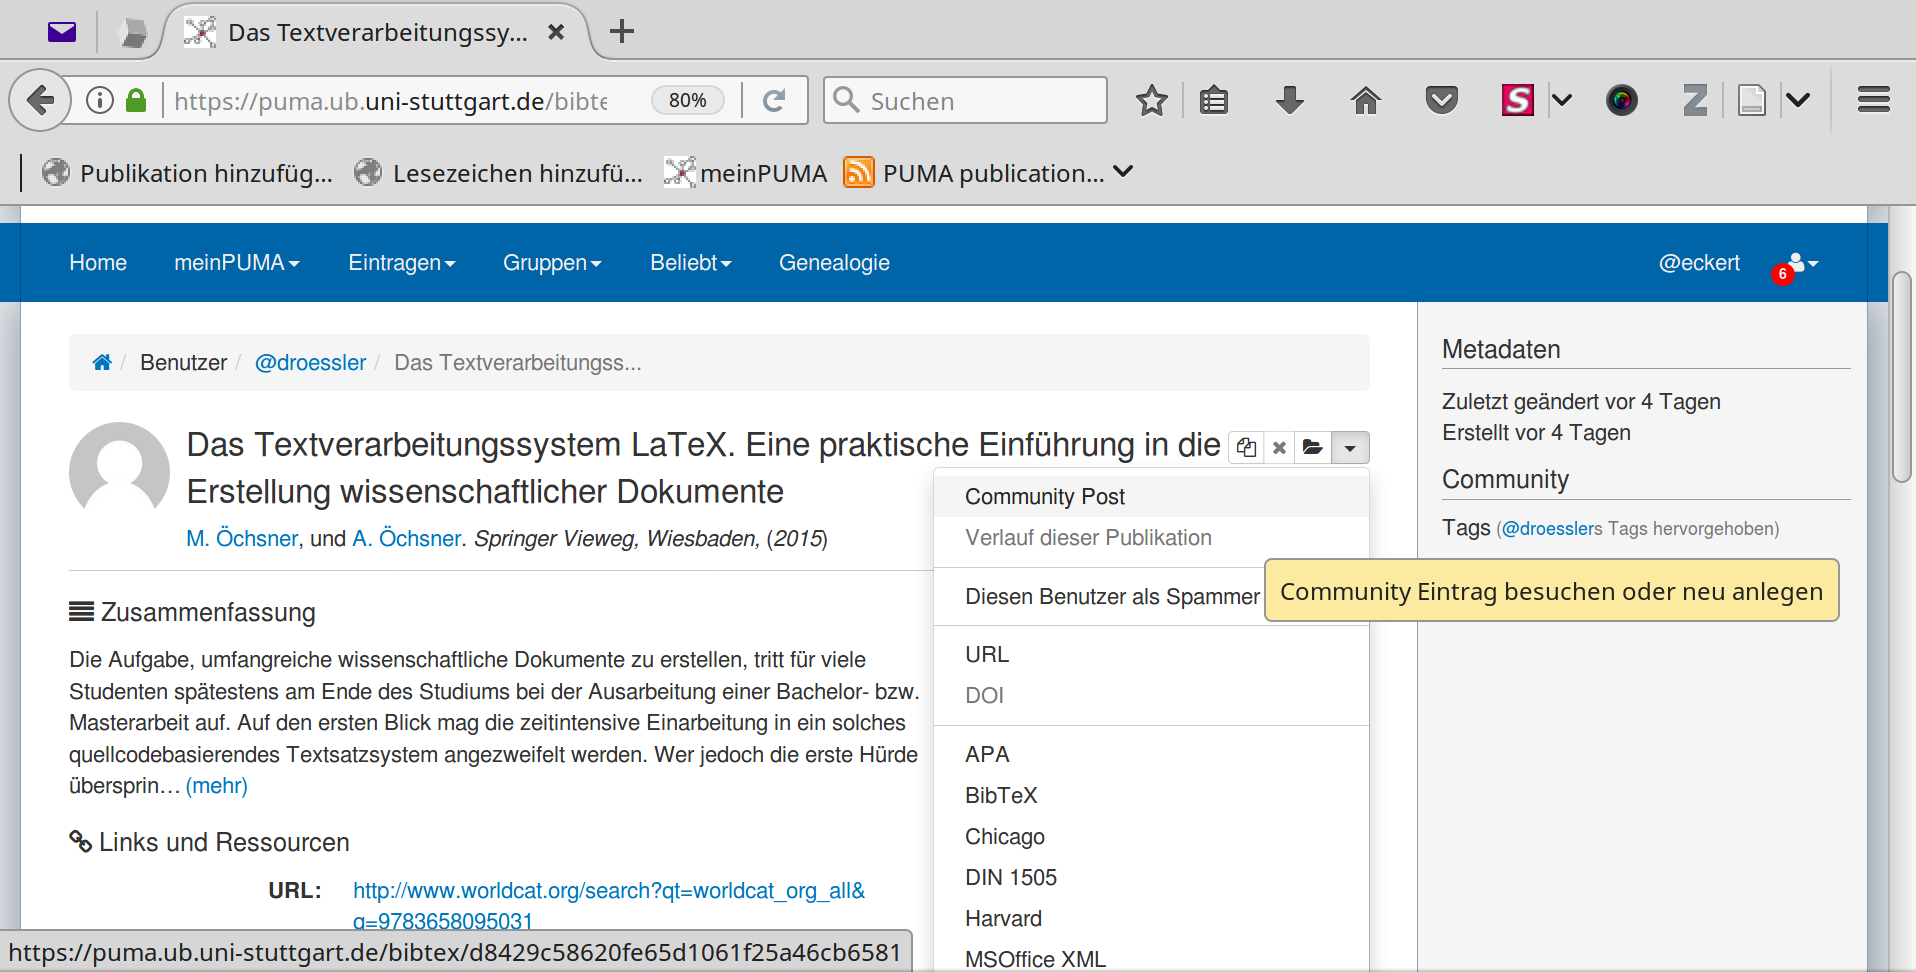
\includegraphics[width=11cm]{Bilder/Kapitel8/Community_post_anlegen}}
 \caption{Community Post anlegen}
 \label{fig:communityPostAnlegen}
\end{figure}
Änderungen an der Publikation können von allen vorgenommen werden, der ursprüngliche Eintrag in der Sammlung des Nutzers, der den Eintrag angelegt hat, ändert sich dabei nicht. Änderungen können über die Versionsgeschichte\index{Versionierung} nachvollzogen werden. 
\todo[inline]{neue Funktionen beschreiben}

Unter dem Bereich \textit{Nutzer} werden alle Nutzer angezeigt, die diese Publikation in Ihrer Sammlung eingetragen haben.
\begin{figure}[h!]
 \centering
 \fbox{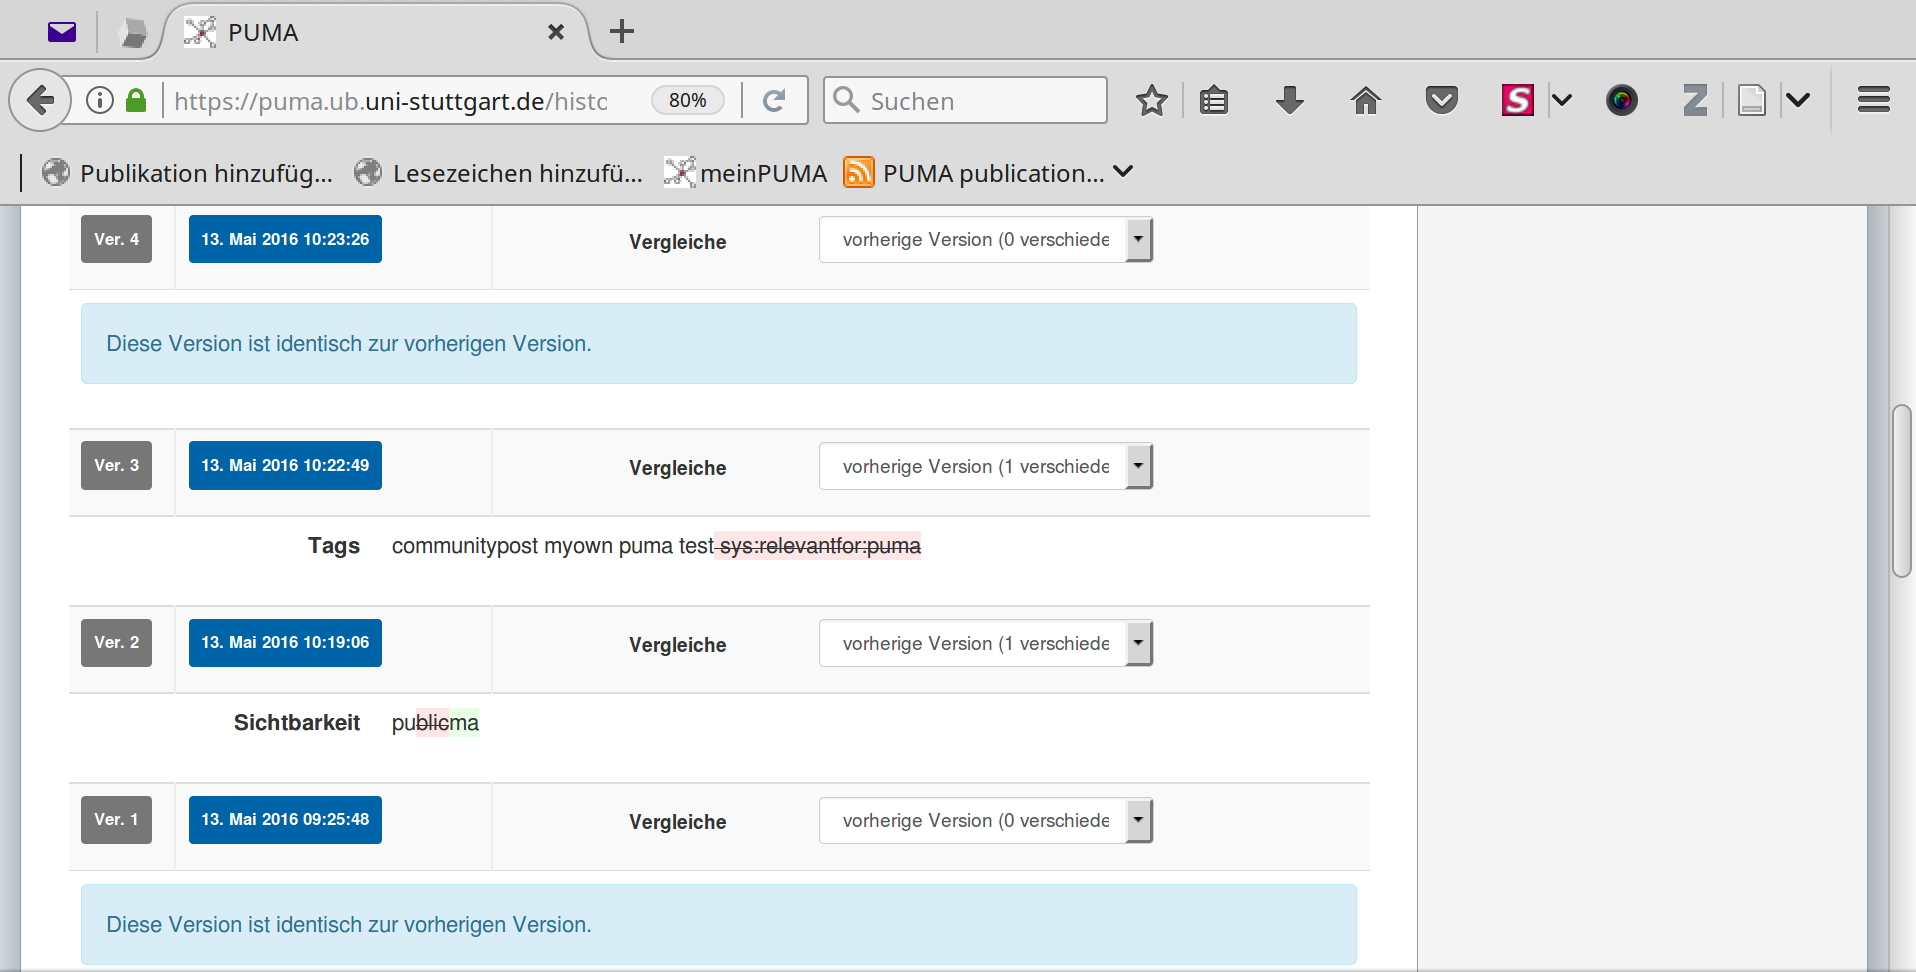
\includegraphics[width=11cm]{Bilder/Kapitel8/Community_post_Versionsgeschichte}}
 \caption{Versionierung}
 \label{fig:versionierung}
\end{figure}
\section{Nutzern folgen}
\label{sec:nutzernFolgen}
Wie in sozialen Netzwerken bietet PUMA die Möglichkeit, anderen Nutzern zu folgen. 

Auf der Benutzerseite (\autoref{subsec:freundHinzu}) unterhalb des Benutzerprofilbildes, auf das Feld \enquote{folgen} klicken. Man kann jedem Nutzer folgen, egal ob man mit ihm befreundet ist oder nicht. \\
Um eine Überblick über die Einträge dieser Person zu erhalten, im Reiter \enquote{meinPUMA} (\autoref{subsec:meinPuma}) auf den Unterpunkt \enquote{verfolgte Einträge} gehen. Es erscheint eine Übersichtsseite mit allen Einträgen der Nutzer, denen man folgt. 




%Überarbeiten:neue version anders

\section{Kommentare, Rezensionen und Bewertungen}
\label{sec:kommentare}
PUMA verfügt über die Möglichkeit, Publikationen und Lesezeichen zu bewerten\index{Bewerten} und Rezensionen\index{Rezensionen} zu verfassen. Man kann mit anderen Nutzern über Publikationen/~Lesezeichen diskutieren und durch die Vergabe von Sternen Publikation und Lesezeichen bewerten.\\
Publikationen/Lesezeichen bewerten:
Dazu auf die Stern-Leiste (siehe \autoref{fig:sternenleiste}) unterhalb des Lesezeichens oder der Publikation klicken.
\begin{figure}[h!]
 \centering
 \fbox{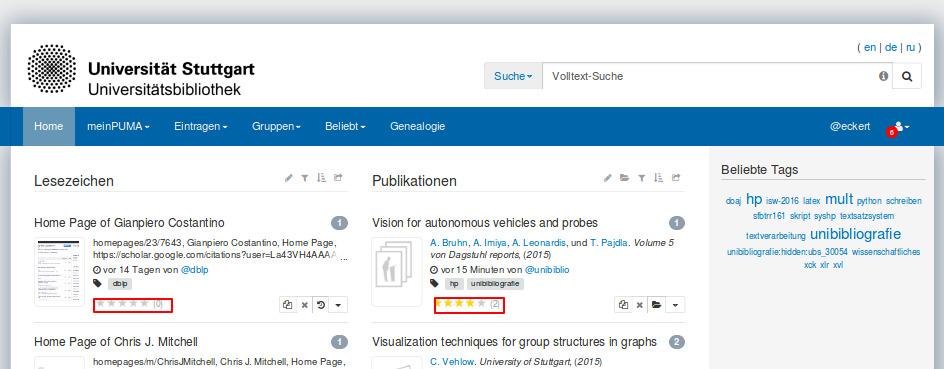
\includegraphics[width=11cm]{Bilder/Kapitel8/Die_Sternenleiste}}
 \caption{Die Stern-Leiste}
 \label{fig:sternenleiste}
\end{figure}  
Es öffnet sich die Gemeinschaftsseite des Eintrages. Neben den Bereichen \textit{Tags} und \textit{Zitieren Sie diese Publikation} findet sich hier auch der Bereich \textit{Kommentare und Rezensionen}. \autoref{fig:publikationBewerten} zeigt die Elemente des Bereichs:
\begin{figure}[h!]
 \centering
 \fbox{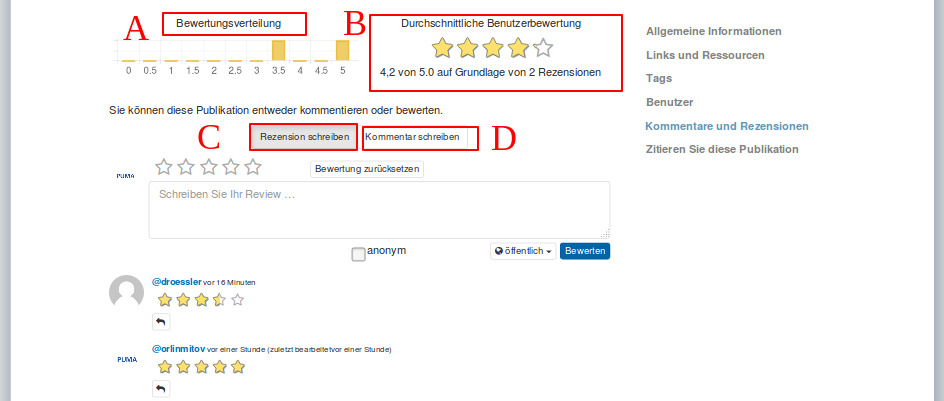
\includegraphics[width=11cm]{Bilder/Kapitel8/Publikation_bewerten}}
 \caption{Publikation bewerten}
 \label{fig:publikationBewerten}
\end{figure}
    \begin{description} 
        \item [Bewertungsverteilung (A):] Das Balkendiagramm stellt dar, welche Bewertungen wie oft vergeben wurden.  %In diesem Fall ... Beispiel an Hand eines Bildes
        \item [Durchschnittliche Bewertung (B):] In der Stern-Leiste wird der Mittelwert der Bewertungen angezeigt.
        \item [Rezension schreiben (C):] \hfill \\
				Durch einen Klick auf den Button "Rezension schreiben" öffnet sich ein Textfeld, das die Möglichkeit bietet, ein Review zu verfassen. Oberhalb des Textfeldes kann der Beitrag mit null bis fünf Sternen bewertet werden. Je höher die Anzahl der Sterne, umso besser ist die Bewertung. Unterhalb des Textfeldes kann die Sichtbarkeit der Bewertung festgelegt werden. Es gibt folgende Möglichkeiten:
        \begin{itemize}
            \item öffentlich: Jeder Nutzer kann die Rezension sehen.
            \item privat: Nur man selber kann die Rezension sehen.
            \item Freunde: Freunde können die Rezension sehen.
            \item Gruppen: Es können alle Gruppen ausgewählt werden, in denen man Mitglied ist.
            \item anonym: Der Kommentar wird ohne Benutzernamen veröffentlicht. Die Bewertung ist für alle Nutzer sichtbar.
        \end{itemize}
     Mit \enquote{Bewerten} kann die Rezension abgeschlossen werden.
             \item [Kommentar schreiben (D):] \hfill \\
				In diesem Textfeld kann auch ein Kommentar verfasst werden. Ein Kommentar hat die gleichen Möglichkeiten der Sichtbarkeit wie die Rezension.\\
Es kann beliebig oft auf Kommentare/~Bewertungen mit Kommentaren reagiert und geantwortet werden. Neben jedem Kommentar befindet sich ein Button mit einem kleinen schwarzen Pfeil, über den die Rezensionen oder ein anderer Kommentar direkt kommentiert werden kann. 
    \end{description}

\todo[inline]{Wichtig: Es wird unterschieden zwischen Rezensionen (mit Bewertungen) und Kommentaren (ohne Bewertungen). Jeder Nutzer kann genau eine Rezension zu einem Artikel verfassen, aber beliebig viele Kommentare. Rezensionen und Kommentare können jederzeit vom Nutzer bearbeitet und gelöscht werden.}